% Software License Agreement
%
% Author    Mike Purvis <mpurvis@clearpathrobotics.com>
% Copyright (c) 2014, Clearpath Robotics, Inc., All rights reserved.
%
% Redistribution and use in source and binary forms, with or without modification, is
% not permitted without the express permission of Clearpath Robotics.


\documentclass[]{clearpath-latex/clearpath-manual}
\graphicspath{{gen/}}
\usepackage{multirow}
\usepackage{gensymb}
\usepackage{dcolumn}
\usepackage{colortbl}
\usepackage{array}


\begin{document}

\manualcover{cover-page.pdf}
\tableofcontents

\section{Introduction}
Clearpath Robotics Kingfisher is a rugged and easy-to-use Unmanned Surface Vessel (USV) for research and rapid prototyping applications. This guide contains information about the setup, operation, and maintenance of your Kingfisher USV.

\subsection{What's Included}

Included with each Kingfisher are the following:

\begin{itemize}[nolistsep]
	\item 1x Clearpath Robotics Kingfisher
	\item 2x 14.4V NiMH Battery Pack
	\item 1x Battery Pack Charger
	\item 1x Futaba Backup Remote Control (R/C)
	\item 1x Payload Connector Dummy Plug
	\item 1x Payload Connector Adapter Kit (plug and pins)
	\item 1x Ethernet Connector Adapter Kit
\end{itemize}

Each Kingfisher deployment (one or more Kingfisher vessels) also includes:

\begin{itemize}[nolistsep]
	\item Clearpath Robotics Base Station
	\item Base Station Battery
	\item Base Station Battery Charger
\end{itemize}

\subsection{What's Required}

The embedded PC onboard Kingfisher runs Ubuntu Linux 12.04 and ROS Hydro. For maximum simplicity, a development computer should be running the same operating system as the onboard computer; however, any version of Ubuntu supported by ROS Hydro will be adequate. If a laptop option was purchased with Kingfisher it will have been already configured with ROS and the appropriate ROS packages. For assistance setting up the development computer, please see the PC Setup section on page \pageref{pcsetup}.

Kingfisher may also be driven using the included Futaba R/C controller as described in the Getting Started section on page \pageref{gettingstarted}. However, the R/C controller is intended as a backup to allow powered retrieval of Kingfisher in case of a PC or network malfunction while on the water. It has significantly reduced range and reliability compared with the standard high-power wireless radio.

\section{The Basics}
This section provides an overview of the key specifications of the Kingfisher platform. \autoref{kf_the_basics} gives a tour of Kingfisher's major components.

\begin{figure}[h]
  \centering
  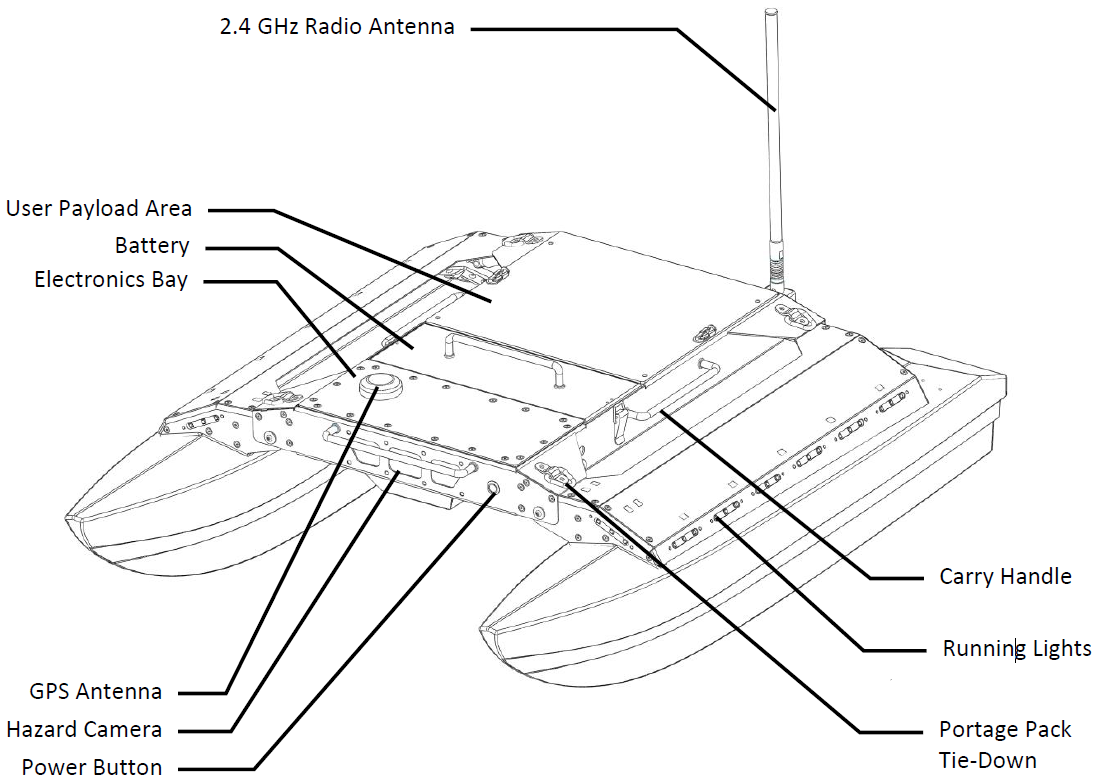
\includegraphics[width=0.75\linewidth]{kf_schematic.PNG}
  \caption{Kingfisher at a Glance (actual boat may vary slightly from image shown)}
  \label{kf_the_basics}
\end{figure}
\newpage

\subsection{Hardware Architecture}
\autoref{kf_architechure} gives an overview of the standard devices which make up Kingfisher. This diagram is provided to aid the user in understanding how Kingfisher is architected.

\begin{figure}[h]
  \centering
  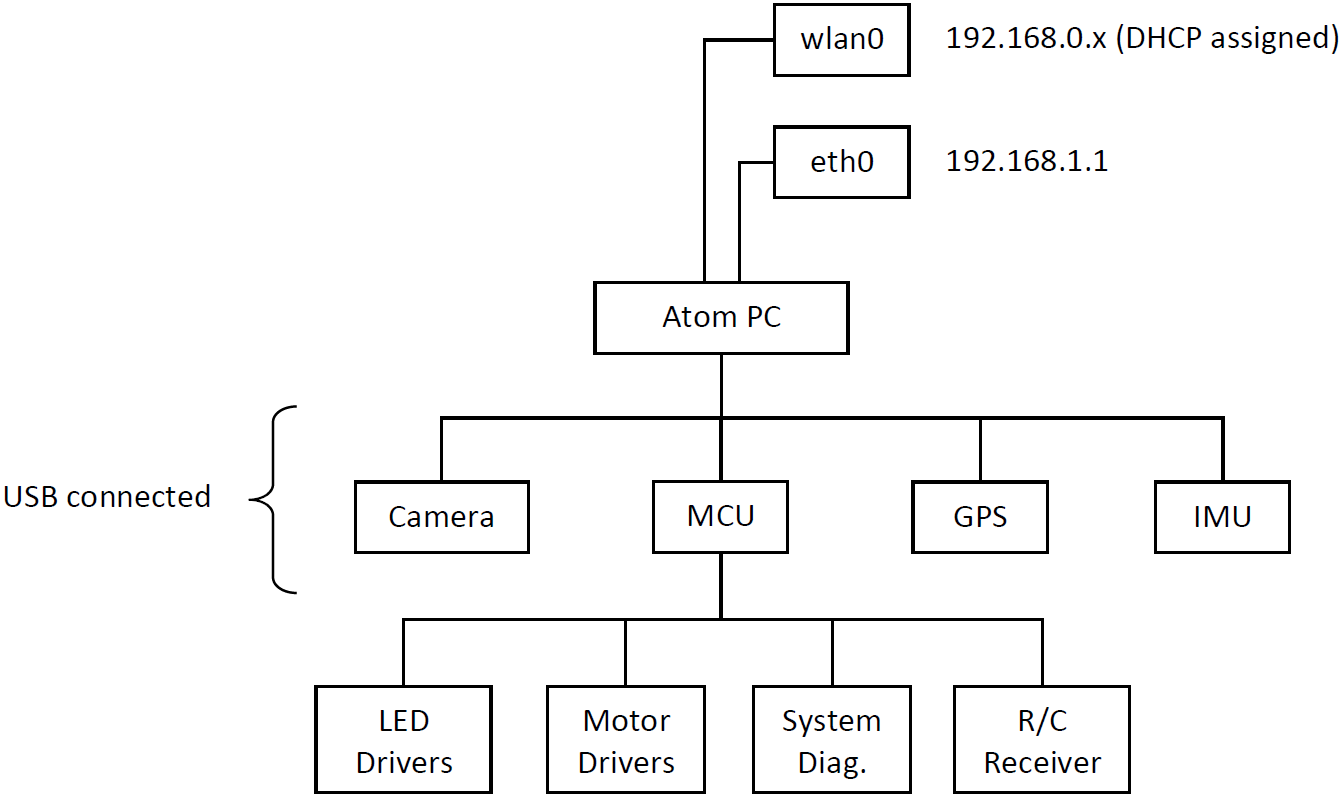
\includegraphics[width=0.75\linewidth]{kf_architecture.PNG}
  \caption{Kingfisher Architecture}
  \label{kf_architechure}
\end{figure}


The etho interface is connected to a weatherproof connector in the User Payload Area. This connector is used to connect Ethernet payloads, such as an IP camera or LIDAR, but may also be used to connect to the vehicle over SSH, especially to adjust the wireless configuration (for example, to change the wireless password, or to associate with a different base station).
\newpage
\subsection{Status Indicators} \label{statusindicators}
The red and green running lights on the port and starboard sides of Kingfisher indicate vehicle status based on the frequency and pattern of flashing. These patterns are described in \autoref{kfstatusindicator}.

\bgroup
\def\arraystretch{1.5}%
\begin{table}[h]
\centering
\begin{tabular}{m{.25\textwidth} p{.6\textwidth}}
\rowcolor{lightgrey} 
Light Pattern     & Description                                                                                                                                                                                              \\ \hline
Solid             & \textbf{No errors}. PC and wireless are active, and a command stream is being received and processed.                                                                                                             \\ \hline
Slow Single Pulse & \textbf{No command}. Indicates that the system is fully up, but the thrusters are not active due to an absence of command messages. Command messages must be sent at 10Hz or faster to maintain steady operation. \\ \hline
Slow Double Pulse & \textbf{Wireless Error}. Indicates that the onboard PC is unable to find the base station’s wireless network. If this indication is seen, check the battery level and indicator lights in the base station.       \\ \hline
Slow Triple Pulse & \textbf{Computer Error}. Indicates that the microcontroller in Kingfisher cannot see the onboard PC. This is expected for about two minutes when first powering on, while the computer boots up.                  \\ \hline
Fast Single Pulse & \textbf{Manual Override}. Indicates that manual control by the Futaba R/C controller is active, and any commands originating from the PC will be disregarded.                                                     \\ \hline
Fast Double Pulse & \textbf{Critical Battery Pack}. Indicates that the system battery level is at or below 13V. Return to shore immediately. \\ \hline                                                                                      
\end{tabular}
\newline
\caption{Kingfisher Status Indicators} 
\label{kfstatusindicator} 
\end{table}
\egroup

The precedence order in the table is downward—that is, the bottom-most condition which is true will be what is indicated by the lights.

\newpage
\subsection{R/C Controller}
Kingfisher ships with a Futaba R/C transmitter integrated as a means of backup control. The intention is always to operate with PC control, but for scenarios where the PC or network malfunctions it is convenient to have an alternate means of retrieving Kingfisher. It’s recommended to remove all AA batteries and store them in a cool dry location when the R/C controller is not in use.

\begin{figure}[h]
  \centering
  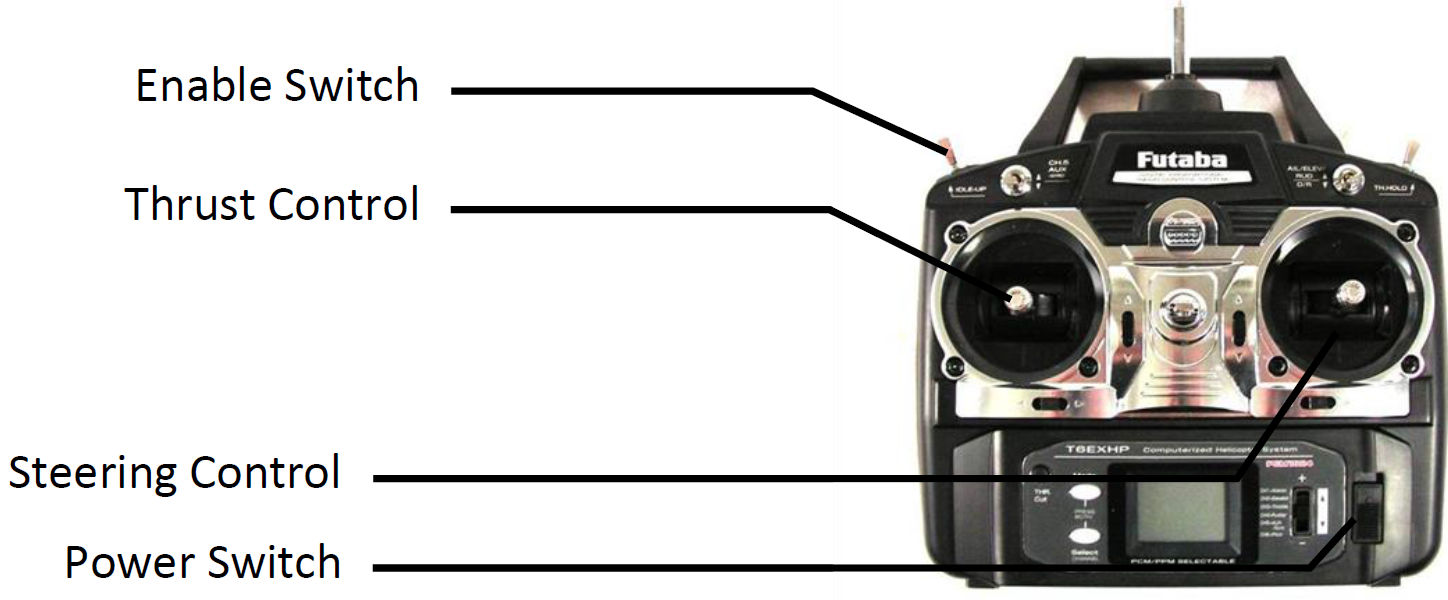
\includegraphics[width=0.75\linewidth]{kf_futaba.PNG}
  \caption{Futaba R/C Transmitter}
  \label{kf_futaba}
\end{figure}

Please see Backup R/C Operation on page \pageref{backupoperation} for details of operating Kingfisher with the RC controller.

\newpage

\subsection{System Specifications}
Key specifications of Kingfisher are shown in \autoref{systemspecs}.

\bgroup
\def\arraystretch{1.2}%
\begin{table}[h]
	\centering
	\begin{tabular}{>{\columncolor{lightgrey}}>{\raggedright}m{.25\textwidth} p{.25\textwidth} p{.25\textwidth}} \hline 
	& 1300 mm length & 51.2 in length \\
	& 940 mm width & 37 in width \\
	\multirow{-3}{*}{Deployed Dimensions} 
	& 340 mm height & 13.4 in height \\ \hline
	
	& 1300 mm length & 51.2 in length \\
	& 550 mm width & 21.6 in width \\
	\multirow{-3}{*}{Stowed Dimensions} 
	& 340 mm height & 13.4 in height \\ \hline
	Chassis Weight (no battery) & 20 kg & 44 lbs \\ \hline
	Battery Weight & 9 kg & 20 lbs \\ \hline
	Draft & 150 mm & 5.9 in \\ \hline
	Maximum Payload & 10 kg & 22 lbs \\ \hline
	Rated speed (forward) & 1.7 m/s & 5.6 ft/s \\ \hline
	& 2.5 hours typical  \\
	\multirow{-2}{*}{Operating Time} 
	& \multicolumn{2}{p{.5\textwidth}}{10 hours standby (no motion)} \\ \hline
	& 14.4V 29 Ah \\
	\multirow{-2}{*}{Battery Pack}
	& NiMH \\ \hline
	Battery Pack Charger & \multicolumn{2}{p{.5\textwidth}}{Short-circuit, over-current, over-voltage, and reverse voltage protection.} \\ \hline
	Charge Time & 10 hours \\ \hline
	User Power & \multicolumn{2}{p{.5\textwidth}}{12V fused at 2.5A} \\ \hline
	Communication & \multicolumn{2}{p{.5\textwidth}}{USB, TCP/IP, RS232, RS485} \\ \hline
	Standard Sensing & \multicolumn{2}{p{.5\textwidth}}{Battery Voltage, GPS, IMU, Hazard Camera} \\ \hline
	
	
	\end{tabular}
\newline
\caption{Kingfisher System Specifications}
\label{systemspecs}
\end{table}
\egroup


\newpage

\section{Safety}
Clearpath Robotics is committed to the safety of our users. Please be advised that Kingfisher is research equipment designed for prototyping applications and we are not able to protect operators, observers, and equipment from all possible use cases. This section provides guidelines to help ensure the safety of personnel and equipment, but the ultimate responsibility lies with the operator.

\subsection{General Warnings}
Kingfisher is a rugged and high-performance vehicle. For the safety of yourself and others, conduct initial experiments in an area that is clear of obstacles and deeper than 0.6 m [24 in]. Although Kingfisher is able to operate in very shallow water, this will avoid any possibility of running aground.

Indoor swimming pools provide an ideal environment for initial testing.

When starting out, it is recommended to favor slower speeds. Operating at speeds lower than 0.5 m/s will give the user more time to react if things don’t go quite as expected.

Adhere to all pool and open water safety considerations.

\begin{warning}
Never operate the Kingfisher in a pool or other bodies of water while people are in the water.}
\end{warning}

\subsection{Electrical System}
Kingfisher is powered by a single 14.4V Nickel-Metal Hydride (NiMH) Battery Pack, the same battery chemistry found in many electric RC cars and boats. Please observe the following precautions:

\begin{itemize}[nolistsep]
	\item Do not tamper with the plug attached to the Battery Pack.
	\item Do not tamper with the Battery Pack connection on Kingfisher.
	\item Do not operate Kingfisher without the Battery Pack clamped securely in position.
	\item Do not tamper with the Electronics Bay.
	\item Charge the Battery Pack only with chargers provided by Clearpath Robotics.
	\item Return the Battery Pack to Clearpath Robotics for proper disposal.
\end{itemize}

\textbf{The Battery Pack has a rugged exterior to protect it from bumps and scrapes, but it still stores a large amount of electrochemical energy and is inherently dangerous. Observe the above precautions carefully.}

\subsection{Lifting and Transport}
For the safety of users and to maximize the lifetime of Kingfisher, please observe the following when manually transporting the robot:

\begin{itemize}[nolistsep]
	\item Kingfisher should be lifted using only the four carrying handles on the vehicle itself. Do not lift Kingfisher by the handle on the Battery Pack.
	\item The Portage Pack accessory is recommended for transporting Kingfisher medium and longer distances.
	\item Ensure that Kingfisher is powered off and the Battery Pack is removed when transporting longer distances.
\end{itemize}

\newpage

\section{Getting Started} \label{gettingstarted}
You are ready to go! This section details how to get the thrusters spinning.

\subsection{Platform Deployment}
Kingfisher has been designed for easy deployment and rapid transit to and from work sites. The hulls and thrusters stow underneath the chassis to reduce the platform's overall size during transit. Unfolding the hulls is a tool-less operation, and is to be done prior to placing the platform in the water. Please see \autoref{kf_pontoon} and the steps following.

\begin{figure}[h]
  \centering
  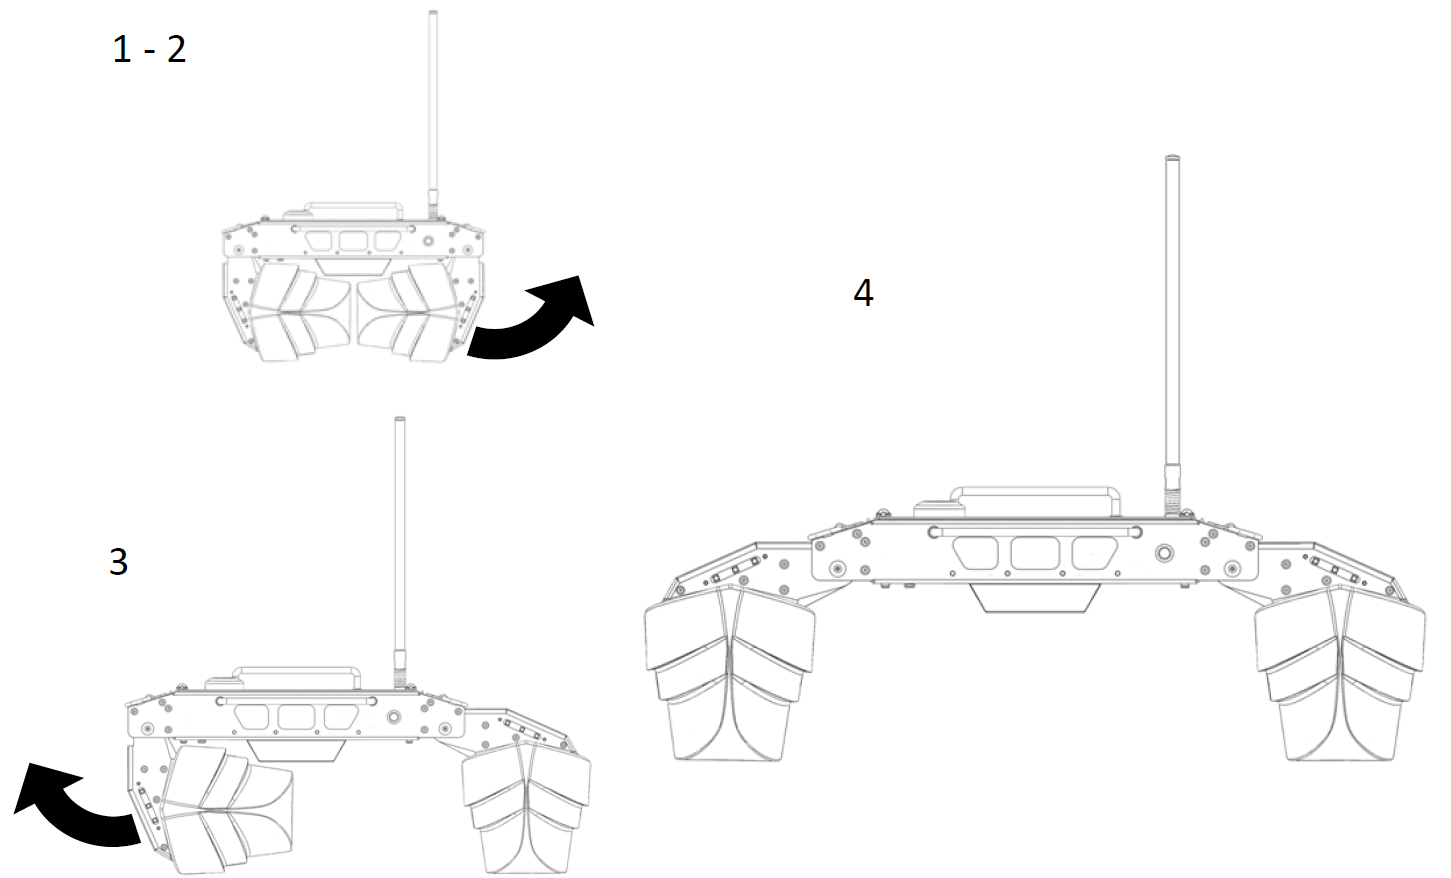
\includegraphics[width=0.75\linewidth]{kf_pontoon.PNG}
  \caption{Pontoon Deployment}
  \label{kf_pontoon}
\end{figure}

\begin{enumerate}[nolistsep]
	\item Place stowed Kingfisher right-side-up on the ground.
	\item Hold the side handle with one hand, and use the other to pull up a stowed hull to the deployment position, setting Kingfisher back down afterward.
	\item Repeat this operation for the opposite hull.
	\item Kingfisher is ready for battery installation and pre-launch check.
\end{enumerate}
\newpage

\subsection{Battery Pack Installation}
Kingfisher comes with a Battery Pack that is discharged and disconnected for safety during shipping. Charge the battery prior to first time use.
To reconnect the Battery Pack, please see \autoref{kf_batteryinstall} and the steps following.

\begin{figure}[h]
  \centering
  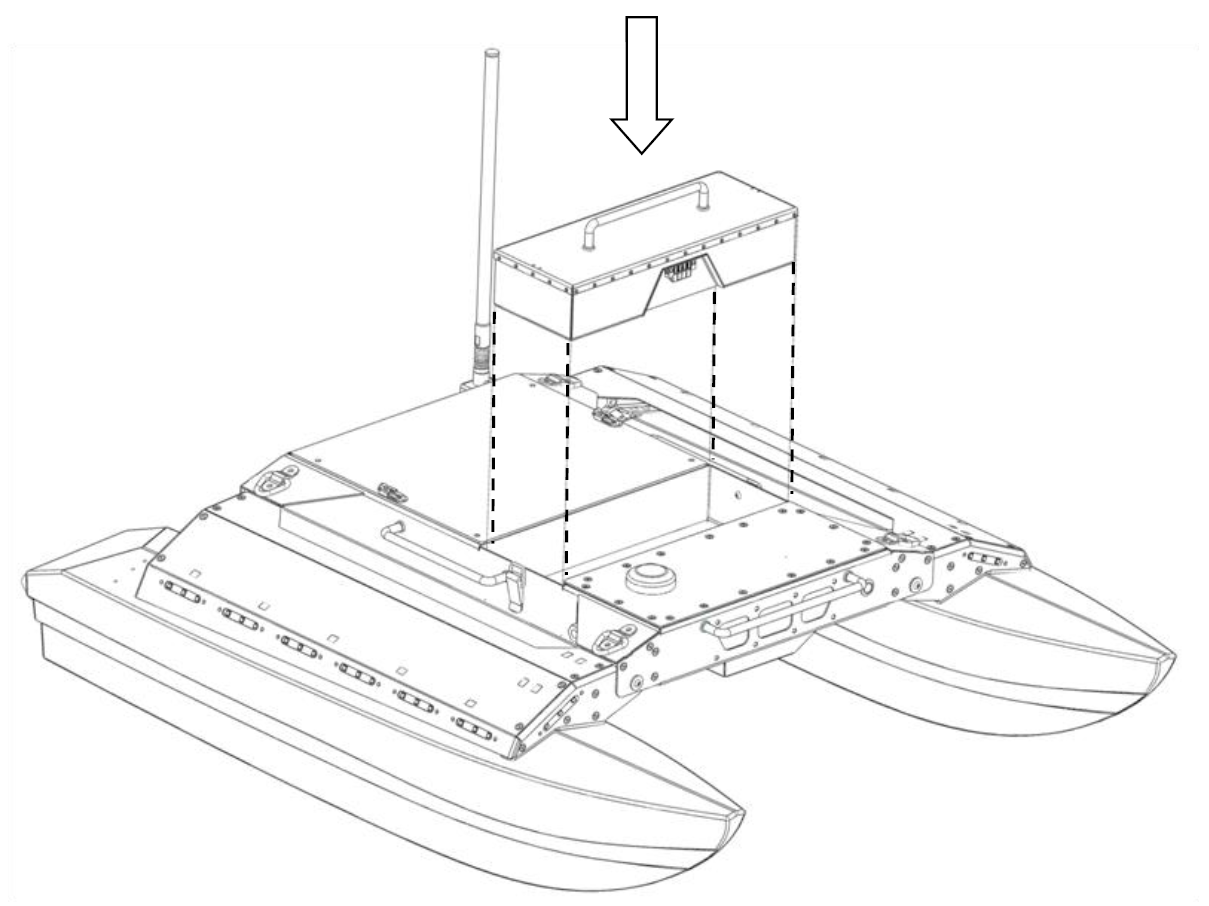
\includegraphics[width=0.75\linewidth]{kf_batteryinstall.PNG}
  \caption{Battery Pack Insertion}
  \label{kf_batteryinstall}
\end{figure}

\begin{enumerate}[nolistsep]
	\item Ensure Kingfisher’s main power button is in the outer “off” position.
	\item Carefully lower the Battery Pack so that the plug is inserted into the mating connector in the Battery Bay. Ensure that it is firmly seated.
	\item Clamp down the latches on either side of the Battery Pack's lid.
\end{enumerate}
\textbf{It is possible to severely damage the battery connector by attempting to insert the battery backwards. Ensure that the battery is oriented correctly before lowering it into the Battery Bay.}
\newpage

\subsection{Powering On}
To power on Kingfisher firmly press the main power button. The power button light will illuminate, and a moment later, the running lights will come on solid for a few seconds before flashing. The motors will play a series of startup chirps to indicate ready status.

For R/C-only operation, the base station is unnecessary. However, if PC operation will be required, set up and power-on the base station as well: Connect the battery to the power supply pigtail, and firmly press the button located on the side of the base station module. A blue LED in the power button will come on, and the radio inside the base station box will light up.

It may take Kingfisher as long as five minutes to find the base station, but when it does, the flashing status indicator should move from Wireless Error (Slow Double Pulse) to No Command (Slow Single Pulse).

Before deploying into water, briefly test the activation of the Kingfisher thrusters with the R/C controller and check wireless connectivity (if required). Do not run the thrusters out of water for more than a few seconds.

\subsection{Backup R/C Operation} \label{backupoperation}
Power-on the R/C controller. Flip the enable switch, top left corner (SW2), down toward the user, which puts Kingfisher in manual override mode. This should be indicated by the Kingfisher running lights moving to short, Fast Single Pulses. Flipping the switch away from the user restores control to the onboard PC.

When operation of the thrusters has been verified on land, deploy Kingfisher into the water and drive it around!

The RC link is much weaker than the main wireless radio link between the Kingfisher and the base station, thus one should expect Kingfisher to go out of R/C range well before losing wireless connectivity. If it is desirable to remain inside R/C range, use ROS on the PC to monitor the /sense topic, which contains a bitfield indicating when the R/C controller is in-range and when it is in control of Kingfisher.

\newpage

\section{ROS Operation}
This section provides an overview of how to use ROS on Kingfisher.

\subsection{PC Setup} \label{pcsetup}

To set up your workstation or laptop (hereafter “development machine”) to work with Kingfisher, begin by following the setup instructions for ROS Hydro: \url{http://wiki.ros.org/hydro/Installation}.

Then, install the Kingfisher ROS stacks:

\begin{lstlisting} 
$ sudo apt-get install ros-hydro-kingfisher-desktop
\end{lstlisting}

At present, this is primarily for the \lstinline{kingfisher_msgs} and \lstinline{kingfisher_teleop packages}. However, the intention is to build this out with display and control interfaces, as well as other software. Please contact Clearpath Robotics support if you have questions about upcoming functionality.

For the most up-to-date version of these instructions, see: \url{http://ros.org/wiki/Robots/Kingfisher}.

\subsection{SSH Connection}
The embedded PC in Kingfisher may be accessed directly, with a wired Ethernet cable, or over the wireless network created by the base station.

For wired access, use a standard Ethernet cable to connect from a laptop to the round Ethernet connector in the User Payload Area. Use your computer’s network configuration utilities to give your Ethernet port an IP in the 192.168.1.x subnet. For example, from the Ubuntu commandline:

\begin{lstlisting}
$ sudo ifconfig eth0 192.168.1.10 up
\end{lstlisting}

Now attempt to ping the onboard computer at its standard IP:

\begin{lstlisting}
$ ping 192.168.1.1
\end{lstlisting}

If successful, you should be ready to connect:

\begin{lstlisting}
$ ssh administrator@192.168.1.1
\end{lstlisting}

The default password is \lstinline{clearpath}.

\textbf{For wireless access}, connect to the base station’s LAN port with an Ethernet cable, or simply join the wireless network (use the credentials included with your shipment). The base station’s administration panel will tell you which IP it assigned to the Kingfisher, or you can use arp or nmap to locate it.

\textbf{To configure the wireless network settings}, first connect via SSH using the wired method above, and then use the WICD network manager. To launch the curses-based interactive text client to WICD, execute:

\begin{lstlisting}
$ wicd-curses
\end{lstlisting}

To give Kingfisher access to the Internet, connect the base station’s WAN port to a wired network connection, or use WICD to temporarily connect Kingfisher to a wireless network with Internet access (such as a wireless hotspot).

\subsection{Developing with the Onboard PC}
When connected to the onboard PC via SSH, be aware of the following locations:

\begin{itemize}[nolistsep]
	\item \textbf{/opt/ros/hydro} is where ROS packages from apt live, including Kingfisher’s core packages. You should not need to modify the contents of this directory.
	\item \textbf{/etc/ros/hydro/kingfisher-core.d} is a directory of roslaunch files which are launched on bootup of Kingfisher’s computer.
\end{itemize}

When you are ready to develop additional software to add to Kingfisher, the recommended path is to add your source repo to a new \lstinline{~/catkin_ws overlay}. When you roslaunch your software, it will seamlessly connect to the already-running background ROS network.

When you’re ready to launch some of your software on boat startup, you can add launchfiles to the \lstinline{kingfisher-core.d} path, but you will also need to change the workspace sourced by the background job. To do this, edit the final line of the \lstinline{/etc/ros/setup.bash} file, and set it to source the setup.bash of the workspace containing the packages which your startup launch file will require.

For more information on using Overlays, see the ROS wiki: \url{http://wiki.ros.org/catkin/Tutorials/workspace_overlaying}

\subsection{ROS Remote Setup}
Connecting with SSH is all well and good, but you often want to be able to run ROS nodes on your development machine and have them able to communicate with the vehicle. This is especially the case with nodes which have a desktop visualization component, such as \lstinline{rviz} or \lstinline{image_view}, or when you want to interface with a locally-connected peripheral, such as the game controller.

The nodes which are launched on startup of Kingfisher have the following environment set:

\begin{lstlisting}
export ROS_IP=192.168.1.1 
export ROS_MASTER_URI=http://$ROS_IP:11311
\end{lstlisting}

When connecting to Kingfisher via the wired Ethernet port, with an IP such as 192.168.1.10 (as instructed above), the setup of the environment on your workstation is indeed simple:

\begin{lstlisting}
export ROS_IP=192.168.1.10 
export ROS_MASTER_URI=http://192.168.1.1:11311
\end{lstlisting}

Once these two commands have been executed on your workstation, it should be possible to run \lstinline{rostopic list, rostopic echo,} etc. to verify that you are communicating with the onboard roscore.

\textbf{What about connecting over wireless?} To get the remote ROS connection over wireless an additional step is required. Say that your development machine is connected to the base station and receives an IP of 192.168.0.120, while the Kingfisher you’d like to communicate with has an IP of 192.168.0.101.

\begin{figure}[h]
  \centering
  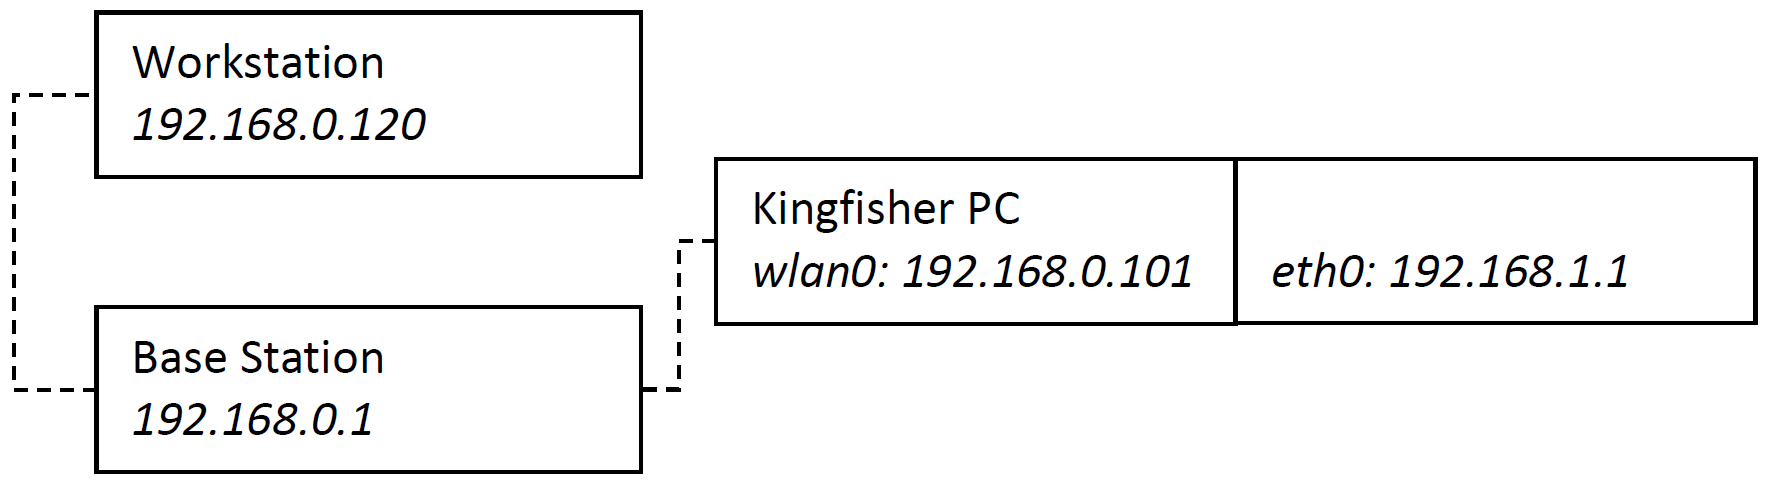
\includegraphics[width=0.75\linewidth]{kf_wireless.PNG}
  \label{kf_wireless}
\end{figure}

The \lstinline{ROS_MASTER_URI} is still the same, but your workstation doesn’t know anything about 129.168.1.1 or where to find it until you give it a little help using the \lstinline{route} command. Execute the following three commands to set up your environment to talk to Kingfisher over the wireless (modify the address of your development machine and the Kingfisher as appropriate, of course):

\begin{lstlisting}
route add -net 192.168.1.1 netmask 255.255.255.255 gw 192.168.0.101 
export ROS_IP=192.168.0.120 
export ROS_MASTER_URI=http://192.168.1.1:11311 
\end{lstlisting}

The route tells your workstation to send packets destined for 192.168.1.1 instead to 192.168.0.101, which is the Kingfisher. Once they’ve made it that far, the Linux networking system will be able to take it from there.

The custom route will not persist between reboots. At any time, you can view the Linux kernel routing table by simply executing:

\begin{lstlisting}
Route
\end{lstlisting}

\subsection{ROS Remote Teleoperation}

When the developer machine has been correctly configured for remote ROS, it should be possible to plug in a standard USB joystick and launch Kingfisher teleoperation:

\begin{lstlisting}
roslaunch kingfisher_teleop joystick_teleop.launch
\end{lstlisting}

This will launch, locally on the development machine, the standard ROS joystick driver, and a translation node which converts joystick messages into velocity command messages. Hold button 1 on your joystick to enable command messages to be sent.

\pagebreak

\subsection{Key Topics}
Kingfisher ships with a rich suite of standard hardware. Each included peripheral is set up from the get-go with appropriate driver software on the onboard PC. This section details how to find the various topics related to each device.

When connected via SSH, or by setting up remote ROS (as detailed above), list available topics with:

\begin{lstlisting}
$ rostopic list
\end{lstlisting}

The \textbf{drive system} publishes information about battery voltage and motor current on the \lstinline{/sense} topic. It listens for commands on \lstinline{/cmd_vel} (geometry\_msgs/Twist) and \lstinline{/cmd_drive} (kingfisher\_msgs/Drive).

The \textbf{IMU} publishes data on the \lstinline{/imu/data} topic.

The \textbf{GPS} publishes fixes on the \lstinline{/gps/fix} topic.

The front-facing hazard camera publishes on the \lstinline{/camera/image_color} suite of image topics. To quickly view the camera feed, execute the following from the development machine: 

\begin{lstlisting}
rosrun image_view image_view image:=/camera/image_color compressed
\end{lstlisting}

\newpage

\section{Payload Integration}
The User Payload Area of Kingfisher includes a standard Ethernet connector, and a custom connector, shown in \autoref{kf_custompayload}, which may be used to power and communicate with serial payloads such as sonar-based instruments.

\textbf{When the mating connectors are not being used the supplied plug connector and dust cap must be installed to ensure that the Kingfisher electronics remain sealed.}

The mating part to the Ethernet connector is the CONEC 17-10001, and the mating part to the custom connector is Amphenol MA1CAE1700, both are available online, for example, from \url{http://mouser.com}.

\begin{figure}[h]
  \centering
  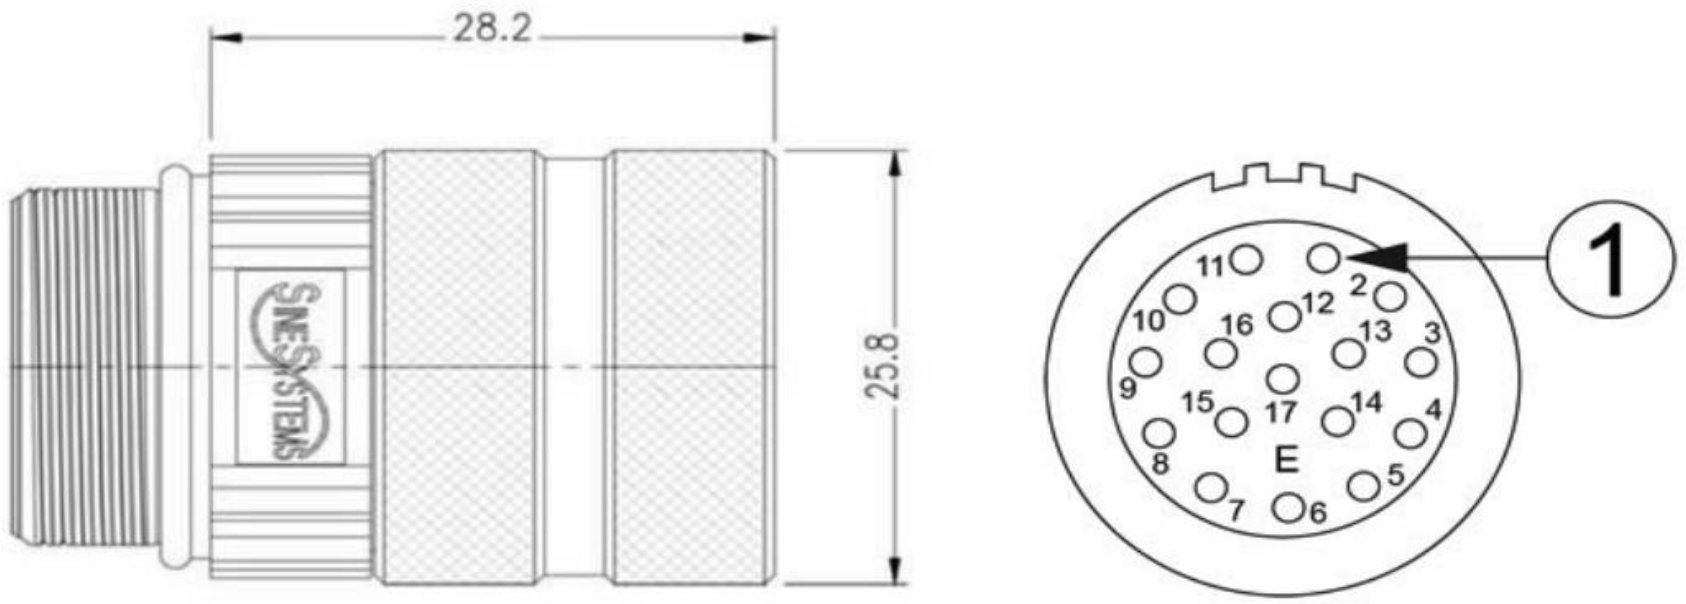
\includegraphics[width=0.75\linewidth]{kf_custompayload.PNG}
  \label{kf_custompayload}
  \caption{Custom Payload Connector Diagram}
\end{figure}

The pinout for this connector is as follows:
\bgroup
\def\arraystretch{1.5}%
\begin{table}[h]
\centering
\label{my-label}
\begin{tabular}{|l|l|} 
\hline
\rowcolor{lightgrey} 
1  & NC              \\ \hline
2  & USER2 RS232 RX  \\ \hline
3  & USER1 RS232 TX  \\ \hline
\rowcolor{lightgrey} 
4  & NC              \\ \hline
5  & GND             \\ \hline
\rowcolor{lightgrey} 
6  & NC              \\ \hline
7  & USER2 RS232 RTS \\ \hline
8  & USER1 RS232 CTS \\ \hline
9  & 12V Supply      \\ \hline
\end{tabular}
\quad
\begin{tabular}{|l|l|} 
\hline
10 & 12V Supply      \\ \hline
11 & 12V GND         \\ \hline
12 & 12V GND         \\ \hline
13 & USER1 RS232 RX  \\ \hline
14 & USER2 RS232 TX  \\ \hline
15 & GND             \\ \hline
16 & USER1 RS232 RTS \\ \hline
17 & USER2 RS232 CTS \\ \hline
\end{tabular}
\end{table}
\egroup

For building the connector, please find assembly instructions online: \url{http://www.sineco.com/assets/images/PDFs/AssemblyInstructions-M23ASeries.pdf}

\newpage

\section{Maintenance}
Kingfisher is built for rugged, long-term use. However, there are steps that can be taken to maintain and extend the life of the platform even further.

\subsection{Charging}
The Battery Pack which ships with Kingfisher can be charged with the following steps:

\begin{enumerate}[nolistsep]
	\item Remove Battery Pack from platform.
	\item Connect the DC output cable from the charger to the Battery Pack terminal connector.
	\item Plug the charger power cord into the charger, and then into a wall receptacle.
	\item Set the Battery Type to NiMH.
	\item Press the 'Start' button, and set the charging current between 2 and 4 amperes.
	\item Hold the 'Start' button for 2 seconds. The charger will play a series of beeps to indicate charging has started.
	\item When the Battery Pack is fully charged, the LCD display will flash 'FULL'. Unplug the charger from the wall, and then disconnect it from the Battery Pack.
\end{enumerate}

Charging at a lower current will require more time, but will ensure that all cells within the Battery Pack are properly balanced, yielding longer runtimes and better overall battery health. It is recommended that each Battery Pack is charged at 2A after every 5 charge-discharge cycles.

\subsection{Battery Pack}
Kingfisher’s power supply is a sealed 14.4 V nickel metal hydride (NiMH) battery, providing 29 ampere-hours of charge. To maximize the lifetime of the Battery Pack, recharge immediately after use, and keep charged to prevent loss in capacity.

The Battery Pack should never be used or stored in an environment exceeding 40 degrees Celsius (104 °F), and should always be charged at temperatures above freezing.

\subsection{Electronics Bay}
Kingfisher's electronics are enclosed in a sealed compartment. These do not require maintenance, and the bay should only be opened by, or under the supervision of, Clearpath Robotics.

\newpage

\section{Tips and Troubleshooting}
This section lists a few possible issues which may be encountered in the course of using Kingfisher.

\bgroup
\def\arraystretch{1.5}%
\begin{table}[h]
\centering
\label{troublshooting}
\begin{tabular}{p{.2\textwidth} p{.7\textwidth}}

\rowcolor{lightgrey} 
{\bf Observation}                    & {\bf Issue \& Resolution}                                                                                                                                                                                                                                                                                          \\ \hline
No power LED                         & \textbf{System is unpowered}. Ensure power button is pressed, and check that battery is properly seated in battery bay. It is unlikely that the battery would be so discharged as to be unable to illuminate the LED, but you could also confirm with a multimeter that the battery has a terminal voltage of at least 14V. \\ \hline
Running lights indicate error status & \textbf{System is in error}. Please refer to Status Indicators on page \pageref{statusindicators} to determine the status being indicated, and contact support for further assistance.                                                                                                                                                               \\ \hline
Can’t ping onboard PC                & \textbf{Network problem}. Ensure that Kingfisher is indicating successful connection to the base station, and that the user laptop is also successfully connected (ie, able to ping 192.168.0.1).                                                                                                                           \\ \hline
Unable to list ROS topics            & \textbf{ROS network problem}. Ensure that the user laptop has a working ROS installation, including the Kingfisher workspace. Ensure that ROS\_MASTER\_URI is correctly pointing to the Kingfisher IP, and that ROS\_IP is set to the user laptop’s IP.                                                                     \\ \hline
Unable to echo ROS topics            & \textbf{ROS environment problem}. Ensure that the user laptop is able to ping Kingfisher, and that ROS\_MASTER\_URI and ROS\_IP are set correctly.                                                                                                                                                                          \\ \hline
\end{tabular}
\end{table}
\egroup

If you’re having some trouble that you don’t see here, or the suggested solution isn’t working out, please get in touch so we can help you with it (see next page for contact details).

For more details on setting up multiple machines to work together in ROS, please see the following pages on the ROS wiki:

\begin{itemize}[nolistsep]


	\item \url{http://www.ros.org/wiki/ROS/NetworkSetup}
	\item \url{http://www.ros.org/wiki/ROS/Tutorials/MultipleMachines}
\end{itemize}

\newpage

\section{Service and Support}
Clearpath is committed to your success with Kingfisher. Please get in touch with us and we'll
do our best to get you rolling again quickly: \href{mailto:support@clearpathrobotics.com}{support@clearpathrobotics.com}
or visit out knowledge base for at \href{http://support.clearpathrobotics.com}{support.clearpathrobotics.com}

To get in touch with our sales team regarding Kingfisher or other Clearpath Robotics products, please
email \href{mailto:sales@clearpathrobotics.com}{sales@clearpathrobotics.com}.

If you have a an issue that is specifically about ROS and is something which may be of interest
to the broader community, consider asking it on \href{http://answers.ros.org}{answers.ros.org}.
If you don't get a satisfactory response, please ping us and include a link to your question
as posted there. If appropriate, we'll answer in the ROS Answers context for the benefit of the
community.

\end{document}
